%	-------------------------------------------------------------------------------
%
%
%
%
%
%
%
%
%	-------------------------------------------------------------------------------

%	\documentclass[10pt,xcolor=pdftex,dvipsnames,table]{beamer}
%	16:10
%	\documentclass[ aspectratio=1610, 10pt,blue,xcolor=pdftex,dvipsnames,table,handout]{beamer}
%	\documentclass[ aspectratio=1610, 10pt,blue,xcolor=pdftex,dvipsnames,table,handout,notes]{beamer}
%	16:9 
%	\documentclass[ aspectratio=169,  10pt,blue,xcolor=pdftex,dvipsnames,table,handout]{beamer}
	\documentclass[ aspectratio=169,  10pt,blue,xcolor=pdftex,dvipsnames,table,handout,notes]{beamer}
%	14:9 
%	\documentclass[ aspectratio=149,  10pt,blue,xcolor=pdftex,dvipsnames,table,handout]{beamer}
%	5:4
%	\documentclass[ aspectratio=54,   10pt,blue,xcolor=pdftex,dvipsnames,table,handout]{beamer}
%	4:3 default
%	\documentclass[ aspectratio=43, 10pt,blue,xcolor=pdftex,dvipsnames,table,handout]{beamer}
%	3:2 
% 	\documentclass[ aspectratio=32, 10pt,blue,xcolor=pdftex,dvipsnames,table,handout]{beamer}







		% Font Size
		%	default font size : 11 pt
		%	8,9,10,11,12,14,17,20
		%
		% 	put frame titles 
		% 		1) 	slideatop
		%		2) 	slide centered
		%
		%	navigation bar
		% 		1)	compress
		%		2)	uncompressed
		%
		%	Color
		%		1) blue
		%		2) red
		%		3) brown
		%		4) black and white	
		%
		%	Output
		%		1)  	[default]	
		%		2)	[handout]		for PDF handouts
		%		3) 	[trans]		for PDF transparency
		%		4)	[notes=hide/show/only]

		%	Text and Math Font
		% 		1)	[sans]
		% 		2)	[sefif]
		%		3) 	[mathsans]
		%		4)	[mathserif]

		%	---------------------------------------------------------	
		%	슬라이드 크기 설정 ( 128mm X 96mm )
		%	---------------------------------------------------------	
			\setbeamersize{text margin left=10mm}
			\setbeamersize{text margin right=10mm}

%			% Format presentation size to A4
%			\usepackage[size=a4]{beamerposter}		% A4용지 크기 사용

%			% Format presentation size to A4
%			\setlength{\paperwidth}{297mm}
%			\setlength{\paperheight}{210mm}
%			\setlength{\textwidth}{287mm}
%			\setlength{\textheight}{200mm}   

%			% Format presentation size to A4 길게
			\setlength{\paperwidth}	{210mm}
			\setlength{\paperheight}	{297mm}
			\setlength{\textwidth}		{190mm}
			\setlength{\textheight}	{287mm}   


%			% Format presentation size to A5
%			\usepackage[size=a5]{beamerposter}		% A5용지 크기 사용

%			% Format presentation size to A5
%			\setlength{\paperwidth}	{210mm}
%			\setlength{\paperheight}	{148mm}
%			\setlength{\textwidth}		{190mm}
%			\setlength{\textheight}	{128mm}   

%			% Format presentation size to A5 길게
%			\setlength{\paperwidth}	{148mm}
%			\setlength{\paperheight}	{210mm}
%			\setlength{\textwidth}		{128mm}
%			\setlength{\textheight}	{190mm}   






	%	========================================================== 	Package
			\usepackage{kotex}						% 한글 사용
			\usepackage{amssymb,amsfonts,amsmath}	% 수학 수식 사용
			\usepackage{color}					%
			\usepackage{colortbl}					%










		
		%	---------------------------------------------------------	
		%		유인물 출력 : 출력할대 조정해서 출력 할것
		%	---------------------------------------------------------	

			\usepackage{pgfpages}
%			\pgfpagesuselayout{2 on 1}[letterpaper]
%			\pgfpagesuselayout{4 on 1}[letterpaper]
%			\pgfpagesuselayout{8 on 1}[letterpaper]

%			\pgfpagesuselayout{resize to}[a4paper,landscape,border shrink=5mm]
			\pgfpagesuselayout{resize to}[a4paper,border shrink=5mm]
%			\pgfpagesuselayout{2 on 1}[a4paper,border shrink=5mm]
%			----------------------------------------------------- 출력 시 설정	1
%			\pgfpagesuselayout{2 on 1}[a4paper]
%			\usecolortheme{seagull}	% 휜색
%			----------------------------------------------------- 출력 시 설정	2
%			\pgfpagesuselayout{2 on 1}[a4paper,border shrink=5mm]
%			\usecolortheme{dove}
%			----------------------------------------------------- 
%			\pgfpagesuselayout{4 on 1}[a4paper,border shrink=5mm]
%			\pgfpagesuselayout{8 on 1}[a4paper,border shrink=5mm]

			\usepackage{handoutWithNotes}
%			\pgfpagesuselayout{1 on 1 with notes}[a4paper,border shrink=5mm]
%			\pgfpagesuselayout{2 on 1 with notes}[a4paper,border shrink=5mm]
%			\pgfpagesuselayout{3 on 1 with notes}[a4paper,border shrink=5mm]
%			\pgfpagesuselayout{4 on 1 with notes}[a4paper,border shrink=5mm]

%			\pgfpagesuselayout{2 on 1}[letterpaper]
%			\pgfpagesuselayout{2 on 1}[letterpaper]
%			\pgfpagesuselayout{2 on 1}[letterpaper]

	%		========================================================= 	Theme

		%	---------------------------------------------------------	
		%	전체 테마
		%	---------------------------------------------------------	
		%	테마 명명의 관례 : 도시 이름
%			\usetheme{default}			%
%			\usetheme{Madrid}    		%
%			\usetheme{CambridgeUS}    	% -red, no navigation bar
			\usetheme{Antibes}			% -blueish, tree-like navigation bar

		%	----------------- table of contents in sidebar
%			\usetheme{Berkeley}		% -blueish, table of contents in sidebar
									% 개인적으로 마음에 듬
%			\usetheme{Marburg}			% - sidebar on the right
%			\usetheme{Hannover}		% 왼쪽에 마크
%			\usetheme{Berlin}			% - navigation bar in the headline
%			\usetheme{Szeged}			% - navigation bar in the headline, horizontal lines
%			\usetheme{Malmoe}			% - section/subsection in the headline

%			\usetheme{Singapore}
%			\usetheme{Amsterdam}

		%	---------------------------------------------------------	
		%	색 테마
		%	---------------------------------------------------------	
%			\usecolortheme{albatross}	% 바탕 파란
%			\usecolortheme{crane}		% 전체적으로 노란색 계열
%			\usecolortheme{beetle}		% 바탕 회색
%			\usecolortheme{dove}		% 전체적으로 흰색 ( 출력용으로 적합 : 잉크 절약)
%			\usecolortheme{fly}		% 전체적으로 회색
%			\usecolortheme{seagull}	% 휜색
%			\usecolortheme{wolverine}	& 제목이 노란색
%			\usecolortheme{beaver}

		%	---------------------------------------------------------	
		%	Inner Color Theme 			내부 색 테마 ( 블록의 색 )
		%	---------------------------------------------------------	

%			\usecolortheme{rose}		% 흰색
%			\usecolortheme{lily}		% 색 안 칠한다
%			\usecolortheme{orchid} 	% 진하게

		%	---------------------------------------------------------	
		%	Outter Color Theme 		외부 색 테마 ( 머리말, 고리말, 사이드바 )
		%	---------------------------------------------------------	

%			\usecolortheme{whale}		% 진하다
%			\usecolortheme{dolphin}	% 중간
%			\usecolortheme{seahorse}	% 연하다

		%	---------------------------------------------------------	
		%	Font Theme 				폰트 테마
		%	---------------------------------------------------------	
%			\usfonttheme{default}		
			\usefonttheme{serif}			
%			\usefonttheme{structurebold}			
%			\usefonttheme{structureitalicserif}			
%			\usefonttheme{structuresmallcapsserif}			



		%	---------------------------------------------------------	
		%	Inner Theme 				
		%	---------------------------------------------------------	

%			\useinnertheme{default}
			\useinnertheme{circles}		% 원문자			
%			\useinnertheme{rectangles}		% 사각문자			
%			\useinnertheme{rounded}			% 깨어짐
%			\useinnertheme{inmargin}			




		%	---------------------------------------------------------	
		%	이동 단추 삭제
		%	---------------------------------------------------------	
%			\setbeamertemplate{navigation symbols}{}

		%	---------------------------------------------------------	
		%	문서 정보 표시 꼬리말 적용
		%	---------------------------------------------------------	
%			\useoutertheme{infolines}


			
	%	---------------------------------------------------------- 	배경이미지 지정
%			\pgfdeclareimage[width=\paperwidth,height=\paperheight]{bgimage}{./fig/Chrysanthemum.jpg}
%			\setbeamertemplate{background canvas}{\pgfuseimage{bgimage}}

		%	---------------------------------------------------------	
		% 	본문 글꼴색 지정
		%	---------------------------------------------------------	
%			\setbeamercolor{normal text}{fg=purple}
%			\setbeamercolor{normal text}{fg=red!80}	% 숫자는 투명도 표시


		%	---------------------------------------------------------	
		%	itemize 모양 설정
		%	---------------------------------------------------------	
%			\setbeamertemplate{items}[ball]
%			\setbeamertemplate{items}[circle]
%			\setbeamertemplate{items}[rectangle]


		%	---------------------------------------------------------	
		%	상자 모양새 설정
		%	---------------------------------------------------------	
%			\setbeamertemplate{blocks}[rounded,shadow=true]
%			\begin{block}
%			\begin{theorem}
%			\begin{lemma}
%			\begin{proof}
%			\begin{corollary}
%			\begin{example}
%			\begin{exampleblock}
%			\begin{alertblock}




		\setbeamercovered{dynamic}


		%	---------------------------------------------------------	
		%		Background 
		%	---------------------------------------------------------	

%			\beamersetaveragebackground{yellow!20}
%			\beamertemplatesolidbackgroundcolor{yellow!20}
%			\beamertemplategridbackground [5mm]




		% --------------------------------- 	문서 기본 사항 설정
		\setcounter{secnumdepth}{1} 		% 문단 번호 깊이
		\setcounter{tocdepth}{1} 			% 문단 번호 깊이




		%	---------------------------------------------------------	
		%		배경 색상 지정
		%	---------------------------------------------------------	
				\setbeamercolor{normal text}{bg=red!12}


% ------------------------------------------------------------------------------
% Begin document (Content goes below)
% ------------------------------------------------------------------------------
	\begin{document}
	

			\title{비머 (Beamer)}
			\subtitle{사용설명서}
			\author{김대희}
			\date[2011.11.10]{2015년 1월}
			\institute[KTS]{(주)서영엔지니어링 \texttt{http://symsone.seoyeong.co.kr/}}



	%	==========================================================
	%
	%	----------------------------------------------------------
		\begin{frame}[plain]
		\titlepage
		
		\end{frame}



	%	==========================================================
	%
	%	----------------------------------------------------------
		\begin{frame}[plain]
		\frametitle{목차}
		\note[item]{목차 내용의 출력}

		\tableofcontents


		\end{frame}



	%	==========================================================
	%		page size
	%	----------------------------------------------------------
		\begin{frame}[t]
		\frametitle{Page Size}

			\begin{block} {Page Size}
			The default page size 
			in a beamer presentation is 128mm $\times$ 96mm (a 4:3 aspect ratio) 
			with a font size of 11pt.
			\end{block}


			\begin{block}{Page Size}
			\begin{itemize}
			\item 16:10 : 160mm $\times$ 100mm
			\item 16: 9 : 160mm $\times$ 90mm
			\item 14: 9 : 140mm $\times$ 90mm
			\item  5: 4 : 125mm $\times$ 100mm
			\item  4: 3 : 128mm $\times$ 96mm
			\item  3: 2 : 135mm $\times$ 90mm
			\end{itemize}
			\end{block}


		
%			% 16:10
%		    \beamer@paperwidth 16.00cm%
%		    \beamer@paperheight 10.00cm%
%			% 16:9
%		    \beamer@paperwidth 16.00cm%
%		    \beamer@paperheight 9.00cm%
%			% 14:9
%		    \beamer@paperwidth 14.00cm%
%		    \beamer@paperheight 9.00cm%
%			% 5:4
%		    \beamer@paperwidth 12.50cm%
%		    \beamer@paperheight 10.00cm%
%			% 4:3
%		    \beamer@paperwidth 12.80cm%
%		    \beamer@paperheight 9.60cm%
%			% 3:2
%		    \beamer@paperwidth 13.50cm%
%		    \beamer@paperheight 9.00cm%

			\textbackslash documentclass[aspectratio=169]\{beamer\}


			\note[item]{Note that this slide is boring.}
			\note[item]{Observe that there are no actual bullets here.}
			\note[item]{Future work: add another bullet.}

		\end{frame}

	%	----------------------------------------------------------
	%		A4 용지 사이즈 크기로 slide Frame 크기 설정
	%	----------------------------------------------------------


		\begin{frame}[t]
		\frametitle{Page Size : A4}
		\note[item]{사이즈를 변경 하고자 하는 경우 사용}

			\begin{block} {package}
			\textbackslash usepackage[size=a4]\{beamerposter\}
			\end{block}


			\begin{block}{preamble}
			\begin{itemize}
			\item[]	Format presentation size to A4
			\item[]	\textbackslash setlength\{\textbackslash paperwidth\}\{29.7cm\}
			\item[]	\textbackslash setlength\{\textbackslash paperheight\}\{21.0cm\}
			\item[]	\textbackslash setlength\{\textbackslash textwidth\}\{28.7cm\}
			\item[]	\textbackslash setlength\{\textbackslash textheight\}\{20.0cm\}   
			\end{itemize}
			\end{block}

%			% Format presentation size to A4
%			\setlength{\paperwidth}{29.7cm}
%			\setlength{\paperheight}{21.0cm}
%			\setlength{\textwidth}{28.7cm}
%			\setlength{\textheight}{20.0cm}   

		\end{frame}


	%	==========================================================
	%		Cover title 
	%	----------------------------------------------------------

		\begin{frame}
		\frametitle{Cover title}
		\note{표지 정의}

			\begin{block}{Cover title}
			\begin{itemize}
			\item[] \textbackslash title\{\} 
			\item[] \textbackslash author\{\} 
			\item[] \textbackslash institute\{\} 
			\item[] 
			\item[] \textbackslash begin\{document\}
			\item[] \textbackslash begin\{frame\}
			\item[] \textbackslash titlepage
			\item[] \textbackslash end\{frame\}
			\end{itemize}
			\end{block}


		\end{frame}



	%	==========================================================
	%		Main slide Frame
	%	----------------------------------------------------------

		\begin{frame}{Main Slide frame}

			\begin{block}{Main Slide frame}
			\begin{itemize}
			\item[] \textbackslash section\{Introduction\} 
			\item[] ~~\textbackslash subsection\{History\} 
			\item[] ~~~~\textbackslash begin\{frame\}[options] 
			\item[] ~~~~\textbackslash frametitle\{History\} 
			\item[] ~~~~~... slide contents ... 
			\item[] ~~~~\textbackslash end\{frame\} 
			\end{itemize}
			\end{block}



		\end{frame}

	%	==========================================================
	%		Frame content
	%	----------------------------------------------------------

		\begin{frame}[plain]{Frame content}
			Frame content
		\end{frame}

	%	----------------------------------------------------------
	%		Frame
	%	----------------------------------------------------------
		\begin{frame}
		\frametitle{Frame content}

			\begin{block} {Frame content}
			\begin{enumerate}
			\item Head Line and foot line
			\item Left and right sidebars
			\item logo
			\item Frame title
			\item Background
			\item Content
			\end{enumerate}
			\end{block}

		\end{frame}


	%	----------------------------------------------------------
	%		head line
	%	----------------------------------------------------------
		\begin{frame}
		\frametitle{Frame content : Head line}

			\begin{block} {Head line}
			\end{block}

		\end{frame}

	%	----------------------------------------------------------
	%		Foot line
	%	----------------------------------------------------------
		\begin{frame}
		\frametitle{Frame content : Foot line}

			\begin{block} {Foot line}
			\end{block}

		\end{frame}

	%	----------------------------------------------------------
	%		left and right sidebars
	%	----------------------------------------------------------
		\begin{frame}
		\frametitle{Frame content : left and right sidebars}

			\begin{block} {left and right sidebars}
			\end{block}

		\end{frame}


	%	----------------------------------------------------------
	%		logo
	%	----------------------------------------------------------
		\begin{frame}
		\frametitle{Frame content : logo}

			\begin{block} {logo}
			\end{block}

		\end{frame}

	%	----------------------------------------------------------
	%		Frame title
	%	----------------------------------------------------------
		\begin{frame}
		\frametitle{Frame content : Frame title}

			\begin{block} {Frame title}
			\begin{itemize}
			\item[]	\textbackslash begin\{frame\}
			\item[]	\textbackslash frametitle \{Frame content : Frame title\}
			\item[]	
			\item[]	\textbackslash end\{frame\}
			\end{itemize}
			\end{block}

		\end{frame}


	%	----------------------------------------------------------
	%		Background
	%	----------------------------------------------------------
		\begin{frame}[t]{Frame content : Background}


			\begin{block} {To set solid background color}
			\textbackslash beamersetaveragebackground\{color\} or\\
			\textbackslash beamertemplatesolidbackgroundcolor\{color\}
			\end{block}

%			\beamersetaveragebackground{color}
%			\beamersetaveragebackground{blue!40}
%			\beamersetaveragebackground{yellow!40}
%			\beamertemplatesolidbackgroundcolor{color}
%			\beamertemplatesolidbackgroundcolor{blue!20}
%			\beamertemplatesolidbackgroundcolor{yellow!20}

			\begin{block} {To set gradient background color}
			\textbackslash beamertemplateshadingbackground\{color1\}\{color2\}.\\
			The colors in this slide is \{blue!5\}\{yellow!10\}.
			\end{block}

%			\beamertemplateshadingbackground{blue!5}{yellow!10}

			\begin{block} {To set grid background}
			\textbackslash beamertemplategridbackground [grid space].
			\end{block}

%			\beamertemplategridbackground [5mm]

		\end{frame}

			%	프레임 바깥에서 정의하니까 적용이 됨		
%			\beamertemplategridbackground [5mm]

	%	----------------------------------------------------------
	%		Content
	%	----------------------------------------------------------
		\begin{frame}{Frame content : Content}

			\begin{block} {Content}
			\end{block}

		\end{frame}





	%	==========================================================
	%		Beamer Option for Output
	%	----------------------------------------------------------


	%	----------------------------------------------------------
	%		Beamer Option for Output
	%	----------------------------------------------------------
		\begin{frame}[t]{Beamer Option for Output}

			\begin{block} {Beamer Option for Output}
			\begin{itemize}
			\item	$[$default$]$ PDF screen ( size 128mm $\times$ 96mm)\footnote{ Monitor's 4:3 aspert ratio}
			\item	$[$handout$]$ for PDF handouts.
			\item	$[$trans$]$ for PDF transparency.
			\item	$[$note=hise/show/only$]$ for note. \\Hide notes (default), add note to the PDF screen, or notes only PDF
			\end{itemize}
			\end{block}



		\note{Beamer Option for Output}
		\end{frame}








	%	----------------------------------------------------------
	%		Beamer Option for Output : handout
	%	----------------------------------------------------------

		\begin{frame}[t]
		\frametitle{Beamer Option for Output : handout (유인물 출력) }

			\begin{block} {Printing multiple pages on one with pgfpages}
			\begin{enumerate}
			\item[]	\textbackslash usepackage\{pgfpages\}
			\item[]	
			\item[]	\textbackslash pgfpagesuselayout\{2 on 1\}[letterpaper]
			\item[]	\textbackslash pgfpagesuselayout\{2 on 1\}[a4paper,border shrink=5mm]
			\item[]	\textbackslash pgfpagesuselayout\{4 on 1\}[a4paper,border shrink=5mm]
			\item[]	\textbackslash pgfpagesuselayout\{8 on 1\}[a4paper,border shrink=5mm]

			\end{enumerate}
			\end{block}
		\end{frame}

%			\usepackage{pgfpages}
%			\pgfpagesuselayout{2 on 1}[letterpaper]
%			\pgfpagesuselayout{4 on 1 with notes}[a4paper,border shrink=5mm]

	%	----------------------------------------------------------
	%		Beamer Option for Output : handout
	%	----------------------------------------------------------
		\begin{frame}[t,shrink=10]
		\frametitle{Beamer Option for Output : handout with note (유인물 출력) }

			\begin{block} {handout With Notes}
			\begin{enumerate}
			\item[]	\textbackslash usepackage\{handoutWithNotes\}
			\item[]	
			\item[]	\textbackslash pgfpagesuselayout\{1 on 1 with notes\}[a4paper,border shrink=5mm]
			\item[]	\textbackslash pgfpagesuselayout\{2 on 1 with notes\}[a4paper,border shrink=5mm]
			\item[]	\textbackslash pgfpagesuselayout\{3 on 1 with notes\}[a4paper,border shrink=5mm]
			\item[]	\textbackslash pgfpagesuselayout\{4 on 1 with notes\}[a4paper,border shrink=5mm]

			\end{enumerate}
			\end{block}
		\end{frame}


%			\usepackage{handoutWithNotes}
%			\pgfpagesuselayout{1 on 1 with notes}[a4paper,border shrink=5mm]
%			\pgfpagesuselayout{2 on 1 with notes}[a4paper,border shrink=5mm]
%			\pgfpagesuselayout{3 on 1 with notes}[a4paper,border shrink=5mm]
%			\pgfpagesuselayout{4 on 1 with notes}[a4paper,border shrink=5mm]



















	%	-------------------------------------------------------------------- section
		\section{section-1}
	%	==========================================================
	%
	%	----------------------------------------------------------
		\begin{frame}[c]{슬라이드 배치}
		\begin{columns}

			\begin{column}{.3\textwidth}
				\begin{block} {슬라이드 본문\\ top 배치}
				\textbackslash begin\{frame\}[t]\{ \}
				\end{block}
			\end{column}

			\begin{column}{.3\textwidth}
				\begin{block} {슬라이드 본문\\ center 배치}
				\textbackslash begin\{frame\}[c]\{ \}
				\end{block}
			\end{column}

			\begin{column}{.31\textwidth}
				\begin{block} {슬라이드 본문\\ bottom 배치}
				\textbackslash begin\{frame\}[b]\{ \}
				\end{block}
			\end{column}

		\end{columns}
		\end{frame}



	%	==========================================================
	%		
	%	----------------------------------------------------------
		\begin{frame}[t]{글꼴 설정}

			\begin{block} {글꼴 설정}
			\begin{description}[12345678901234567890]
			\item[\textbackslash emph	\{연습\}] 			\emph{연습} 
			\item[\textbackslash textbf	\{연습\}] 			\textbf{연습} 
			\item[\textbackslash textit	\{연습\}] 			\textit{연습} 
			\item[\textbackslash textsl	\{연습\}] 			\textsl{연습} 

			\item[\textbackslash alert	\{연습\}] 			\alert{연습} 
			\item[\textbackslash textrm	\{연습\}] 			\textrm{연습} 
			\item[\textbackslash textsf	\{연습\}] 			\textsf{연습} 
			\item[\textbackslash color	\{green\}연습]		\color{green}연습
			\end{description}
			\end{block} {}


		\end{frame}



	%	==========================================================
	%		Color
	%	----------------------------------------------------------
		\begin{frame}[t]{Color}

		\begin{columns}[t]
			\begin{column}{.4\textwidth}
				\begin{block} {}
				\begin{description}[1234567890]
				\item	[black] 		{\color{blue!70} A B C }
				\item	[darkgray] 	{\color{darkgray!70} A B C }
				\item	[lime] 		{\color{lime!70} A B C }
				\item	[pink]		{\color{pink!70} A B C }
				\item	[violet]		{\color{violet!70} A B C }
				\item	[blue]		{\color{blue!70} A B C }
				\item	[gray]		{\color{gray!70} A B C }
				\item	[magenta]		{\color{magenta!70} A B C }
				\item	[purple]		{\color{purple!70} A B C }
				\item	[white]		{\color{white!70} A B C }
				\end{description}
				\end{block}
			\end{column}
	
			\begin{column}{.4\textwidth}
				\begin{block} {}
				\begin{description}[1234567890]
				\item	[brown]		{\color{brown!70} A B C }
				\item	[green]		{\color{green!70} A B C }
				\item	[olive]		{\color{olive!70} A B C }
				\item	[red]		{\color{red!70} A B C }
				\item	[yellow]		{\color{yellow!70} A B C }
				\item	[cyan]		{\color{cyan!70} A B C }
				\item	[lightgray]	{\color{lightgray!70} A B C }
				\item	[orange]		{\color{orange!70} A B C }
				\end{description}
				\end{block}
	
			\end{column}
	
		\end{columns}
		\end{frame}




	%	-------------------------------------------------------------------- section
	%	==========================================================
		\section{페이지 배치}

	%	----------------------------------------------------------
	%	이동 단추 삭제
	%	----------------------------------------------------------
		\subsection{이동단축 삭제}
		\begin{frame}{이동단추삭제}

			\begin{block} {\textbackslash setbeamertemplate}
			\textbackslash setbeamertemplate\{navigation symbols\}\{\}
			\end{block}
		\end{frame}


	%	----------------------------------------------------------
	%	배경 이미지 지정
	%	----------------------------------------------------------
		\subsection{배경 이미지 지정}
		\begin{frame}[shrink=0]{배경 이미지 지정}

			\begin{block} {배경 이미지 지정}
			\end{block}
		\end{frame}


	%	----------------------------------------------------------
	%	본문 글꼴색 지정
	%	----------------------------------------------------------
		\subsection{본문 글꼴색 지정}
		\begin{frame}[shrink=0]{본문 글꼴색 지정}

			\begin{block} {본문 글꼴색 지정}
			\end{block}
		\end{frame}



	%	==========================================================
	%	슬라이드가 클 경우 페이지 나누기
	%	----------------------------------------------------------
		\begin{frame}[c]
		\frametitle{슬라이드가 클 경우 페이지 나누기}

			\begin{block} {본문 글꼴색 지정}
			\begin{description}[12345678901234567890]
			\item[allowframebreaks] 알아서 나누기 
			\item[shrink] 화면을 비율로 축소
			\item[] 페이지 나누기 명령
			\end{description}
			\end{block}


		\end{frame}



	%	==========================================================
	%	allowframebreaks
	%	----------------------------------------------------------

		\begin{frame}[c]
		\frametitle{슬라이드가 클 경우 페이지 나누기}

			\begin{block} {allowframebreaks}
			\end{block}


		\end{frame}


	%	==========================================================
	%	shrink
	%	----------------------------------------------------------
		\begin{frame}[shrink=20]{화면 배치 배율 조정 shrink}
			
			\begin{block} {화면 배치 배율 조정 shrink=20}

			\begin{enumerate}
			\item[]	\textbackslash begin\{frame\}[shrink=20]
			\item[]	\textbackslash frametitle\{화면 배치 배율 조정 shrink\}
					본문 첫번째 슬라이드에 들어갈 내용\\
			\item[]	\textbackslash end\{frame\}
			\end{enumerate}

			\end{block}

			The default page size in a beamer presentation is 12.8cm x 9.6cm (a 4:3 aspect ratio) with a font size of 11pt.

		\end{frame}


	%	==========================================================
	%	allowframebreaks
	%	----------------------------------------------------------

		\begin{frame}[c]
		\frametitle{슬라이드가 클 경우 페이지 나누기}

			\begin{block} {페이니 나누기 명령}
			\end{block}


		\end{frame}





















	%	-------------------------------------------------------------------- section
		\section{테마}
	%	==========================================================
	%		테마
	%	----------------------------------------------------------

		\begin{frame}[plain]
		\centering
		\scalebox{8}{themes}
		\end{frame}



%		\subsection{젼체 테마}
	%	==========================================================
	%
	%	----------------------------------------------------------
		\begin{frame}[t]{Five Themes}

			\begin{block} {Five Theme categories}
			\begin{enumerate}
			\item Presentation Themes
			\item Color Themes
			\item Font Themes
			\item Inner Themes
			\item Outer Themes
			\end{enumerate}
			\end{block}

		\end{frame}


	%	----------------------------------------------------------
	%		Presentation	Theme
	%	----------------------------------------------------------
		\begin{frame}[t,shrink=10]{프리젠테이션 테마}

			\begin{block} {프리젠테이션 테마}
			\begin{description}[12345678901234]
			\item [\textbf{default}]
			\item [\textbf{Madrid}]    		
			\item [\textbf{CambridgeUS}] 	- red, no navigation bar
			\item [\textbf{Antibes}] 		- blueish, tree-like navigation bar
			\item [\textbf{Berkeley}]		- blueish, table of contents in sidebar\\
										- 개인적으로 마음에 듬
			\item [\textbf{Marburg}]		- sidebar on the right
			\item [\textbf{Hannover}]		- 왼쪽에 마크
			\item [\textbf{Berlin}]		- navigation bar in the headline
			\item [\textbf{Szeged}]		- navigation bar in the headline, horizontal lines
			\item [\textbf{Malmoe}]		- section/subsection in the headline
			\item [\textbf{Singapore}]
			\item [\textbf{Amsterdam}]
			\end{description}
			\end{block}

		\end{frame}


	%	----------------------------------------------------------
	%		Color Theme
	%	----------------------------------------------------------
		\begin{frame}[t,shrink=10]{color theme}

			\begin{block} {색 테마 : 정의 }
			\begin{itemize}
			\item[] \textbackslash usecolortheme\{albatross\}	\% 바탕 파란
			\end{itemize}
			\end{block}

			\begin{block} {색 테마 : 종류 }
			\begin{description}[12345678901234]
			\item [albatross]	바탕 파란
			\item [crane]		바탕 흰색
			\item [beetle]	바탕 회색
			\item [dove]		전체적으로 흰색
			\item [fly]		전체적으로 회색
			\item [seagull]	휜색
			\item [wolverine]	제목이 노란색
			\item [beaver]
			\end{description}
			\end{block}

		\end{frame}



	%	----------------------------------------------------------
	%		Font Theme
	%	----------------------------------------------------------
		\begin{frame}[t,shrink=10]{Font Theme}

			\begin{block} {\textbackslash usfonttheme }
			\begin{description}[12345678901234]
			\item [default]
			\item [serif]		
			\item [structurebold]
			\item [structureitalicserif]
			\item [structuresmallcapsserif]
			\end{description}
			\end{block}
		\end{frame}



	%	----------------------------------------------------------
	%		Inner Color Theme
	%	----------------------------------------------------------
		\begin{frame}[t,shrink=10]{Inner Color Theme}

			\begin{block} {Inner Color Theme 내부 색 테마 ( 블록의 색 )}
			\begin{description}[12345678901234]
			\item [rose]		흰색
			\item [lily]		색 안 칠한다
			\item [orchid] 	진하게
			\end{description}
			\end{block}

		\end{frame}


	%	----------------------------------------------------------
	%		Outer Color Theme
	%	----------------------------------------------------------
		\begin{frame}[t,shrink=10]{Outter Color Theme}

			\begin{block} {Outter Color Theme 외부 색 테마 ( 머리말, 고리말, 사이드바 )}
			\begin{description}[12345678901234]
			\item [whale]		진하다
			\item [dolphin]	중간
			\item [seahorse]	연하다
			\end{description}
			\end{block}

		\end{frame}




	%	----------------------------------------------------------
	%		Inner Theme
	%	----------------------------------------------------------
		\begin{frame}[t,shrink=10]{Inner Theme}

			\begin{block} {\textbackslash useinnertheme}
			\begin{description}[12345678901234]
			\item [default]
			\item [circles]	 원문자			
			\item [rectangles]	 사각문자			
			\item [rounded]	 깨어짐
			\item [inmargin]		
			\end{description}
			\end{block}
		\end{frame}


	%	----------------------------------------------------------
	%		Outer Theme
	%	----------------------------------------------------------
		\begin{frame}[t]{Outer Theme}

			\begin{block} {\textbackslash Outer Theme}
			\end{block}
		\end{frame}



	%	----------------------------------------------------------
	%		use Outer Theme
	%	----------------------------------------------------------
		\begin{frame}{useoutertheme : 문서 정보 표시 꼬리말 적용}

			\begin{block} {\textbackslash useoutertheme}
			\textbackslash useoutertheme\{infolines\}
			\end{block}
		\end{frame}





	%	-------------------------------------------------------------------- section
		\section{List}
	%	==========================================================
	%		List
	%	----------------------------------------------------------

		\begin{frame}[plain]
		\centering
		\scalebox{10}{List}

		\note{List}
		\end{frame}


	%	==========================================================
	%	itemize	
	%	==========================================================
		\begin{frame}[t]{itemize}

			\begin{block} {itemize}
				\begin{itemize}
				\item 킹
						\begin{itemize}
						\item 킹
								\begin{itemize}
								\item 킹
								\item 왕
								\item 짱
								\end{itemize}
						\item 왕
						\item 짱
						\end{itemize}
				\item 왕
				\item 짱
				\end{itemize}
			\end{block}

		\note{itemize}
		\end{frame}






	%	==========================================================
	%		enunerate
	%	==========================================================
		\begin{frame}[t]{enumerate}

			\begin{block} {enumerate}
			\begin{enumerate}
			\item 킹
					\begin{enumerate}
					\item 킹
							\begin{enumerate}
							\item 킹
							\item 왕
							\item 짱
							\end{enumerate}
					\item 왕
					\item 짱
					\end{enumerate}
			\item 왕
			\item 짱
			\end{enumerate}
			\end{block}


		\note{enumerate}
		\end{frame}




	%	==========================================================
	%	description
	%	==========================================================
		\begin{frame}[t]{description}

		\begin{block} {description}
			\begin{description}
				\item[1 아이템] 1 아이템 설명
				\item[22 아이템] 2 아이템 설명
				\item[333 아이템] 3 아이템 설명
			\end{description}
	
	
			\begin{description}[123456789012345]
				\item[1 아이템] 1 아이템 설명
				\item[22 아이템] 2 아이템 설명
				\item[333 아이템] 3 아이템 설명
			\end{description}
		\end{block}

		\note{description}
		\end{frame}



	%	-------------------------------------------------------------------- section
		\section{Table}
	%	==========================================================
	%		Table
	%	----------------------------------------------------------

		\begin{frame}[plain]
		\centering
		\scalebox{10}{Table}

		\note{Table}
		\end{frame}



	%	==========================================================
	%		Table
	%	----------------------------------------------------------
		\begin{frame}
		\frametitle{table}

			\begin{center}
			\rowcolors{1}{blue!20}{yellow!20}
			% LATEX + dvips에서만 작동	
			\begin{table}
			\caption{Famous Composers}
			\begin{tabular}{ l|c }
				\hline
				J. S. Bach & 1685--1750 \\
				W. A. Mozart & 1756--1791 \\
				L. Beethoven & 1770--1827 \\
				F. Chopin & 1810--1849 \\
				R. Schumann & 1810--1856 \\
				B. Bart’{o}k & 1881--1945 \\ 
				\hline
			\end{tabular}
			\end{table}
			\end{center}
		\end{frame}



		\begin{frame}
		\end{frame}



	%	-------------------------------------------------------------------- section
		\section{수식}
	%	==========================================================
	%		수식
	%	----------------------------------------------------------

		\begin{frame}[plain]
		\centering
		\scalebox{10}{수식}

		\note{수식}
		\end{frame}



	%	==========================================================
	%		수식 넣기
	%	----------------------------------------------------------
		\begin{frame}
		\frametitle{수식 넣기}

			어디서 많이 본 수식 하나
			\[x = \frac{-b \pm \sqrt{b^2 - 14 ac}} { 2a } \]

		\end{frame}



		\begin{frame}
		\end{frame}












	%	-------------------------------------------------------------------- section
		\section{그림}
	%	==========================================================
	%		그림
	%	----------------------------------------------------------

		\begin{frame}[plain]
		\centering
		\scalebox{10}{그림}

		\note{그림}
		\end{frame}

	%	==========================================================
	%		그림 넣기 에제
	%	----------------------------------------------------------
		\begin{frame}
		\frametitle{그림 넣기 예제}
			\begin{figure}
			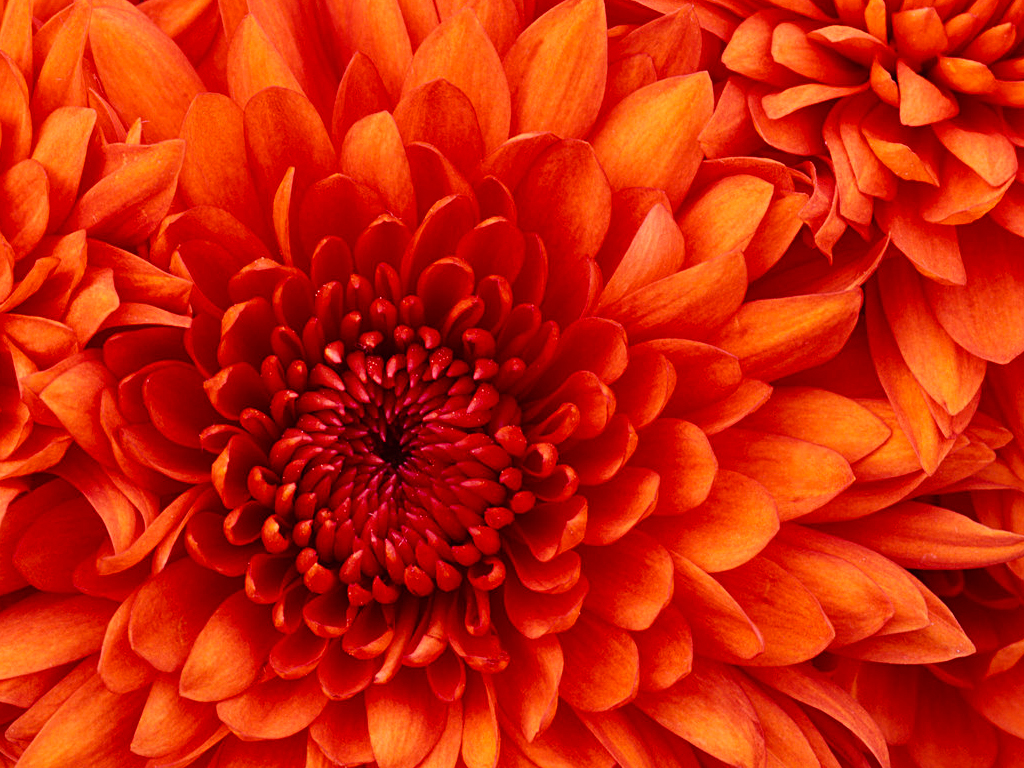
\includegraphics[scale=1.0,width=0.6\textwidth]{./fig/Chrysanthemum.jpg}
			\caption{국화}
			\end{figure}
		\end{frame}




	%	==========================================================
	%		beamer color box
	%	==========================================================
	%		Table
	%	----------------------------------------------------------

		\begin{frame}[plain]
			\structure{beamer color box}
		\end{frame}

	%	----------------------------------------------------------
	%		beamer color box
	%	----------------------------------------------------------

		\begin{frame}[allowframebreaks]

		\null
		\begin{block} {beamer color box}
			\textbackslash begin\{beamercolorbox\} [$<$option$>$] \{ $<$beamer color$>$ \}\\
			$<$ environment contents $>$ \\
			\textbackslash end\{beamercolorbox\}
		\end{block}

		\newpage \null
		\begin{block} {beamer color box}
			\begin{itemize}	
			\item	wd=$<$width$>$
			\item	dp=$<$depth$>$
			\item	ht=$<$height$>$
			\item	left
			\item	right
			\item	center
			\item	leftskip=$<$left skip$>$
			\item	rightskip=$<$right skip$>$
			\end{itemize}
		\end{block}

		\newpage \null
		\begin{block} {beamer color box}
			\begin{itemize}	
			\item	sep=$<$dimension$>$
			\item	colsep=$<$dimension$>$
			\item	colsep*=$<$dimension$>$
			\item	shadow=$<$true or false$>$
			\item	rounded=$<$true or false$>$
			\item	ignorebg
			\item	vmode
			\end{itemize}
		\end{block}

		\end{frame}

		\begin{frame}

			\begin{example}
				\textbackslash setbeamercolor\{postit\}\{fg=black,bg=yellow\} \\
				\textbackslash begin\{beamercolorbox\}[sep=1em,wd=5cm]\{postit\} \\
				~~Place me somewhere! \\
				\textbackslash end\{beamercolorbox\}\\
			\end{example}


			\setbeamercolor{postit}{fg=black,bg=yellow}
			\begin{beamercolorbox}[sep=1em,wd=5cm]{postit}
			Place me somewhere!
			\end{beamercolorbox}

		\end{frame}





	%	-------------------------------------------------------------------- section
		\section{Block}
	%	==========================================================
	%		block
	%	==========================================================


	%	----------------------------------------------------------
	%		block
	%	----------------------------------------------------------


		\begin{frame}[plain]
		\centering
		\scalebox{10}{Block}

		\note{block}
		\end{frame}


	%	Example: \setbeamertemplate{blocks}[default]
	%	Example: \setbeamertemplate{blocks}[rounded][shadow=true]


		

	%	----------------------------------------------------------
	%		Block
	%	----------------------------------------------------------

		\begin{frame}{block}

			\begin{block} {Block}
			\end{block}

			\begin{block} {}
			한글텍학회는 2007년 1월에 창립되었읍니다.	
			\end{block}

		\end{frame}



	%	----------------------------------------------------------
	%		Block : block
	%	----------------------------------------------------------

		\begin{frame}[t]{block}

			\begin{block} {block 제목}
			한글텍학회는 2007년 1월에 창립되었읍니다.	
			\end{block}

			\begin{example}
			한글텍학회는 2007년 1월에 창립되었읍니다.	
			\end{example}

			\begin{alertblock} {alertblock 제목}
			한글텍학회는 2007년 1월에 창립되었읍니다.	
			\end{alertblock}

		\end{frame}

	%	----------------------------------------------------------
	%		Block : theorem
	%	----------------------------------------------------------
		\begin{frame}[t]{theorem}
			\begin{theorem}
			정리 : 한글텍학회는 2007년 1월에 창립되었읍니다.	
			\end{theorem}
		\end{frame}

	%	----------------------------------------------------------
	%		Block : lemma
	%	----------------------------------------------------------
		\begin{frame}[t]{lemma}

			\begin{lemma}
			보조 정리 :  한글텍학회는 2007년 1월에 창립되었읍니다.	
			\end{lemma}

		\end{frame}


	%	----------------------------------------------------------
	%		Block : proof
	%	----------------------------------------------------------
		\begin{frame}[t]{proof}

			\begin{proof}
			증명 : 한글텍학회는 2007년 1월에 창립되었읍니다.	
			\end{proof}

		\end{frame}


	%	----------------------------------------------------------
	%		Block : example
	%	----------------------------------------------------------
		\begin{frame}[t]{example}

			\begin{example} {example}
			한글텍학회는 2007년 1월에 창립되었읍니다.	
			\end{example}

			\begin{example} {}
			한글텍학회는 2007년 1월에 창립되었읍니다.	
			\end{example}

			\begin{example}
			한글텍학회는 2007년 1월에 창립되었읍니다.	
			\end{example}


		\end{frame}


	%	----------------------------------------------------------
	%		Block : alertblock
	%	----------------------------------------------------------
		\begin{frame}[t]{alertblock}

			\begin{alertblock} {주의 ; alertblock}
			한글텍학회는 2007년 1월에 창립되었읍니다.	
			\end{alertblock}

		\end{frame}



	%	==========================================================
	%		Block 	다단 편집
	%	----------------------------------------------------------
		\begin{frame}[t]
		\frametitle{다단 편집하기}

			\begin{example} {다단 편집 top 배치}
			\textbackslash begin\{columns\}[t]
			\end{example}

		\begin{columns}[t]
		\begin{column}{.5\textwidth}
			\begin{block} {항목 나열}
			\begin{itemize}
			\item 첫 번째
			\item 두 번째
			\end{itemize}
			\end{block}

		\end{column}

		\begin{column}{.4\textwidth}
			\begin{block} {그림 삽입}
			\centerline{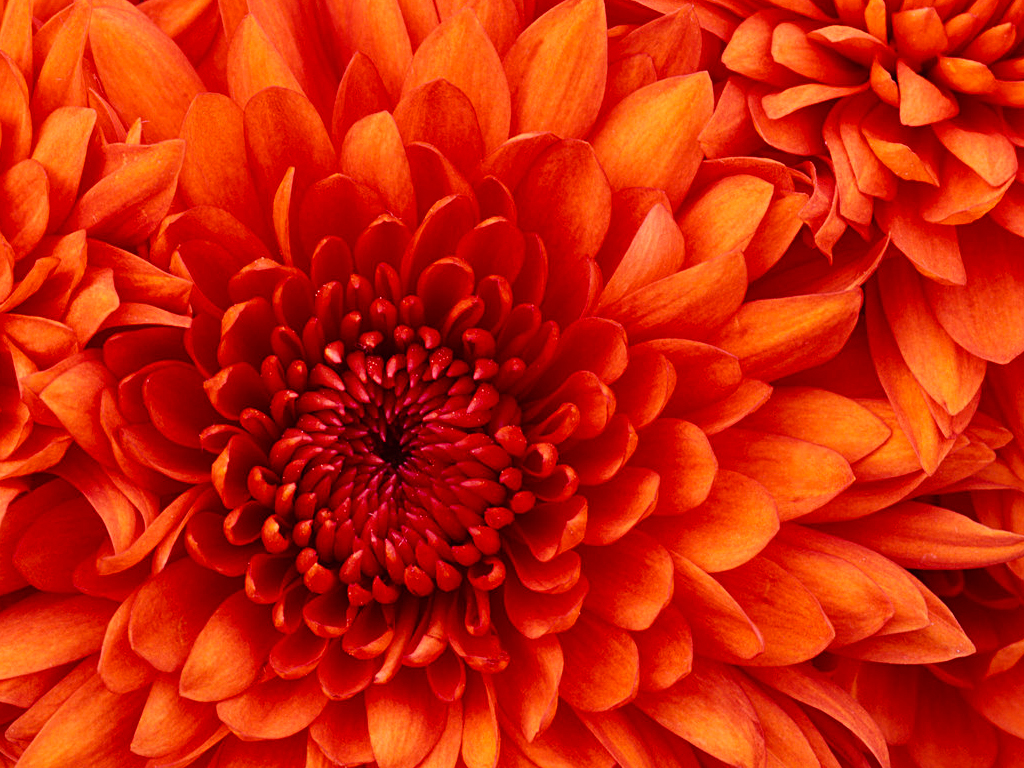
\includegraphics[scale=1.0,width=0.6\textwidth]{./fig/Chrysanthemum.jpg}}
			\end{block}

		\end{column}
		\end{columns}
		\end{frame}

	%	----------------------------------------------------------
	%		Block 	다단 편집
	%	----------------------------------------------------------
		\begin{frame}[t]
		\frametitle{다단 편집하기}

			\begin{example} {다단 편집 center 배치}
			\textbackslash begin\{columns\}[c]
			\end{example} 


		\begin{columns}[c]
		\begin{column}{.5\textwidth}
			\begin{block} {항목 나열}
			\begin{itemize}
			\item 첫 번째
			\item 두 번째
			\end{itemize}
			\end{block}

		\end{column}

		\begin{column}{.4\textwidth}
			\begin{block} {그림 삽입}
			\framebox{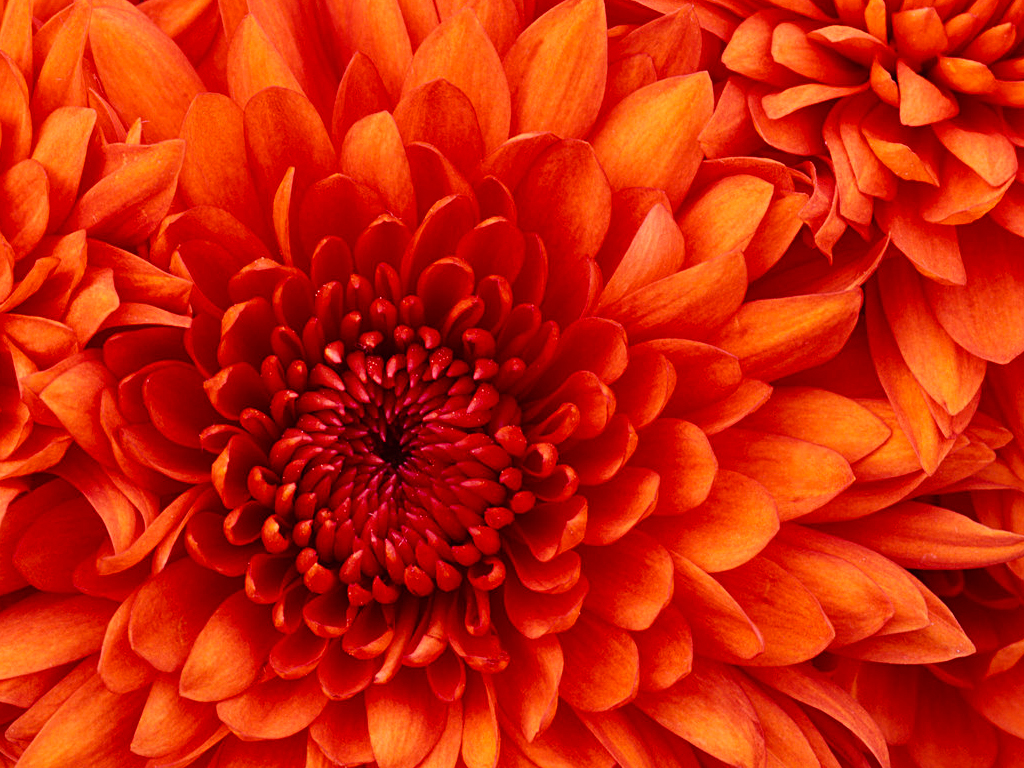
\includegraphics[scale=1.0,width=0.6\textwidth]{./fig/Chrysanthemum.jpg}}
			\end{block}

		\end{column}
		\end{columns}
		\end{frame}




	%	----------------------------------------------------------
	%		Block 	다단 편집
	%	----------------------------------------------------------
		\begin{frame}[t]
		\frametitle{다단 편집하기}

			\begin{example} {다단 편집 bottom 배치}
			\textbackslash begin\{columns\}[b]
			\end{example}

		\begin{columns}[b]
		\begin{column}{.5\textwidth}

			\begin{block} {항목 나열}
			\begin{itemize}
			\item 첫 번째
			\item 두 번째
			\end{itemize}
			\end{block}

		\end{column}

		\begin{column}{.4\textwidth}

			\begin{block} {그림 삽입}
			\centerline{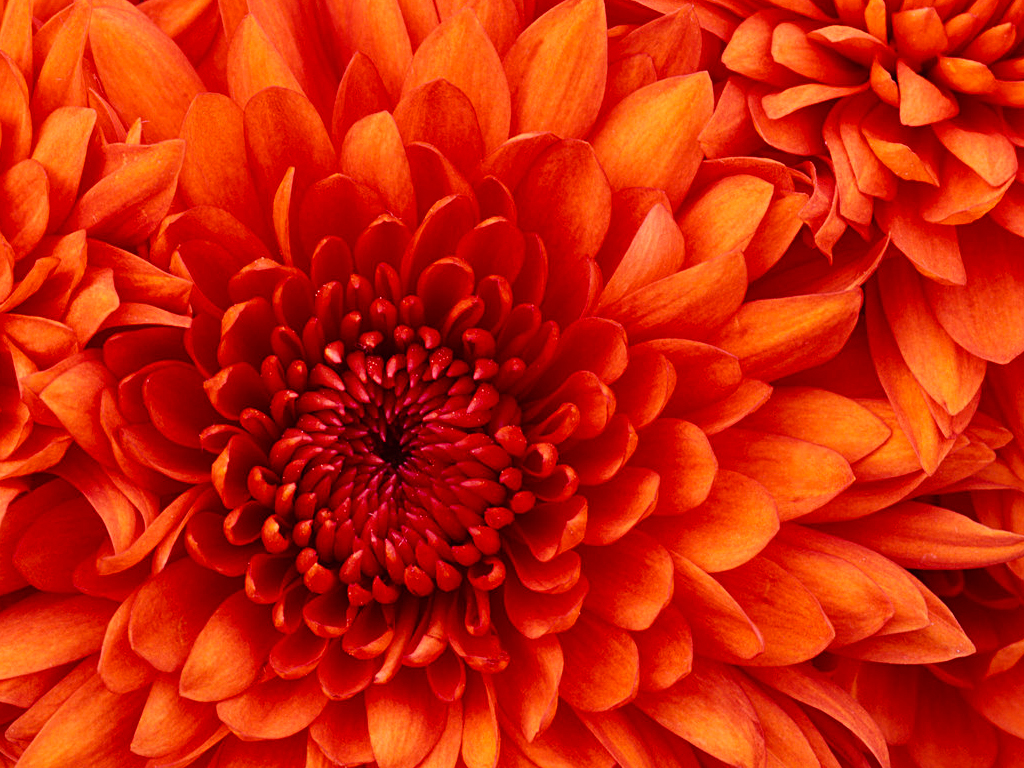
\includegraphics[scale=1.0,width=0.6\textwidth]{./fig/Chrysanthemum.jpg}}
			\end{block}

		\end{column}
		\end{columns}
		\end{frame}






	%	-------------------------------------------------------------------- section
		\section{오버레이 연습} 
	%	==========================================================
	%		오버레이 연습
	%	----------------------------------------------------------

		\begin{frame}[plain]
		\centering
		\scalebox{5}{오버레이 연습}

		\note{오버레이 연습}
		\end{frame}


	%	----------------------------------------------------------
	%
	%	----------------------------------------------------------
		\begin{frame}[t]{오버레이}

		슬라이드 쇼의 기본값은 각 슬라이드가 한번에 모두 나타나게 하는 것이다.
		그러나 마우스 클릭을 하때마다 항목이 순차적으로 나타나게 하는 것이 효과적일때가 많다.
		실제로는 클릭수 만큼의 문서를 생성하여 마치 클릭할때마다 항목이 나타나는 것처럼 보이게 처리한다. 
		이를 오버레이(overlay)라고 한다. 가장 단순한 것으로는 명령어 \textbackslash pause가 있다.


		\end{frame}

	%	----------------------------------------------------------
	%
	%	----------------------------------------------------------
		\begin{frame}[t]{오버레이 연습}

			\begin{block} {하나씩만 나타나기 $<$ 1 $>$ }
			\begin{enumerate}
			\item <1> 1 킹
			\item <2> 2 킹
			\item <3> 3 킹
			\item <4> 4 왕
			\item <5> 5 짱
			\end{enumerate}
			\end{block} 

		\end{frame}

	%	----------------------------------------------------------
	%
	%	----------------------------------------------------------
		\begin{frame}[t]{오버레이 연습}

			\begin{block} {하나씩만 나타내다 마지막에 전체표시\\
						$<$ 1, 마지막+1 $>$ }
			\begin{enumerate}
			\item <1,6> 1 킹
			\item <2,6> 2 킹
			\item <3,6> 3 킹
			\item <4,6> 4 왕
			\item <5,6> 5 짱
			\end{enumerate}
			\end{block} 

		\end{frame}




	%	----------------------------------------------------------
	%
	%	----------------------------------------------------------
		\begin{frame}[t]{오버레이 연습}

			\begin{block} {하나씩 순차적으로 나타나기 $<$ n - $>$ }
			\begin{enumerate}
			\item <1-> $<$1-$>$ 킹
			\item <2-> $<$2-$>$ 킹
			\item <3-> $<$3-$>$ 킹
			\item <4-> $<$4-$>$ 왕
			\item <5-> $<$5-$>$ 짱
			\end{enumerate}
			\end{block}

		\end{frame}


	%	----------------------------------------------------------
	%
	%	----------------------------------------------------------
		\begin{frame}[t]{오버레이 연습}

			\begin{block} {하나씩 순차적으로 없어지기 $<$ - 1 $>$}
			\begin{enumerate}
			\item <-1> $<$-1$>$ 킹
			\item <-2> $<$-2$>$ 킹
			\item <-3> $<$-3$>$ 킹
			\item <-4> $<$-4$>$ 왕
			\item <-5> $<$-5$>$ 짱
			\end{enumerate}
			\end{block}

		\end{frame}

	%	----------------------------------------------------------
	%
	%	----------------------------------------------------------
		\begin{frame}[t]{오버레이 연습}

			\begin{block} {하나씩 순차적으로 없어졌다, 마지막이 전체 표시\\
						 $<$ - 1, 마지막번호 $>$}
			\begin{enumerate}
			\item <-1,6> $<$-1,6$>$ 킹
			\item <-2,6> $<$-2,6$>$ 킹
			\item <-3,6> $<$-3,6$>$ 킹
			\item <-4,6> $<$-4,6$>$ 왕
			\item <-5,6> $<$-5,6$>$ 짱
			\end{enumerate}
			\end{block}

		\end{frame}



	%	----------------------------------------------------------
	%		일반적인 사용법 -> 순차적으로 나타남
	%	----------------------------------------------------------
		\begin{frame}[t]{오버레이 연습 }

			\begin{block} {일반적인 사용법 $<$ + - $>$}
			\begin{enumerate}
			\item <+-> $<+->$ 1 킹
			\item <+-> $<+->$ 2 킹
			\item <+-> $<+->$ 3 킹
			\item <+-> $<+->$ 4 왕
			\item <+-> $<+->$ 5 짱
			\end{enumerate}
			\end{block}

		\end{frame}



	%	----------------------------------------------------------
	%		일반적인 사용법의 역사용 -> 순차적으로 없어짐
	%	----------------------------------------------------------
		\begin{frame}[t]{오버레이 연습 }

			\begin{block} {일반적인 사용법 $<$ - + $>$}
			\begin{enumerate}
			\item <-+> $<-+>$ 1 킹
			\item <-+> $<-+>$ 2 킹
			\item <-+> $<-+>$ 3 킹
			\item <-+> $<-+>$ 4 왕
			\item <-+> $<-+>$ 5 짱
			\end{enumerate}
			\end{block}

		\end{frame}




	%	----------------------------------------------------------
	%
	%	----------------------------------------------------------
		\begin{frame}[t]{오버레이}

			\begin{block} {오버레이 연습}
			\begin{enumerate}
			\item <1-6> 1 킹
			\item <2-6> \uncover<2>{ 2 킹}
			\item <3-6> 3 킹
			\item <4-6> 4 왕
			\item <5-6> 5 짱
			
			\end{enumerate}
			\end{block}

		\end{frame}




% ------------------------------------------------------------------------------
% End document
% ------------------------------------------------------------------------------
\end{document}


